\setcounter{table}{0}
\renewcommand{\thetable}{S\arabic{table}}

\setcounter{figure}{0}
\renewcommand{\thefigure}{S\arabic{figure}}

\section{Model Specification and Training Details}

\subsection{Atom and Bond Features}
All categorical features are one-hot encoded. Atomic mass is included as a real-valued feature scaled to unit order.
\begin{table}[ht]
\centering
\caption{Atom features used in the D-MPNN encoder.}
\label{tab:atom-features}
\begin{tabular}{lll}
\toprule
\textbf{Feature} & \textbf{Description} & \textbf{Size} \\
\midrule
Atom type & Atomic number–based encoding & 100 \\
Number of bonds & Total bonded neighbors & 6 \\
Formal charge & Integer formal charge & 5 \\
Chirality & Tetrahedral CW/CCW or unspecified & 4 \\
Number of hydrogens & Bonded hydrogen count & 5 \\
Hybridization & sp, sp$^2$, sp$^3$, sp$^3$d, sp$^3$d$^2$ & 5 \\
Aromaticity & Aromatic atom indicator & 1 \\
Atomic mass & Scaled atomic mass & 1 \\
\bottomrule
\end{tabular}
\end{table}

\begin{table}[ht]
\centering
\caption{Bond features used in the D-MPNN encoder.}
\label{tab:bond-features}
\begin{tabular}{lll}
\toprule
\textbf{Feature} & \textbf{Description} & \textbf{Size} \\
\midrule
Bond type & Single, double, triple, aromatic & 4 \\
Conjugation & Conjugated bond indicator & 1 \\
Ring membership & Bond in ring indicator & 1 \\
Stereo & None, any, E/Z, cis/trans & 6 \\
\bottomrule
\end{tabular}
\end{table}

\subsection{Training Convergence Under Fixed Horizons}
Figure~\ref{fig:si-convergence} presents training and validation loss curves for $N=100$ and $N=11{,}816$ to assess whether fixed training horizons induce late-epoch validation divergence.
\begin{figure}
    \centering
    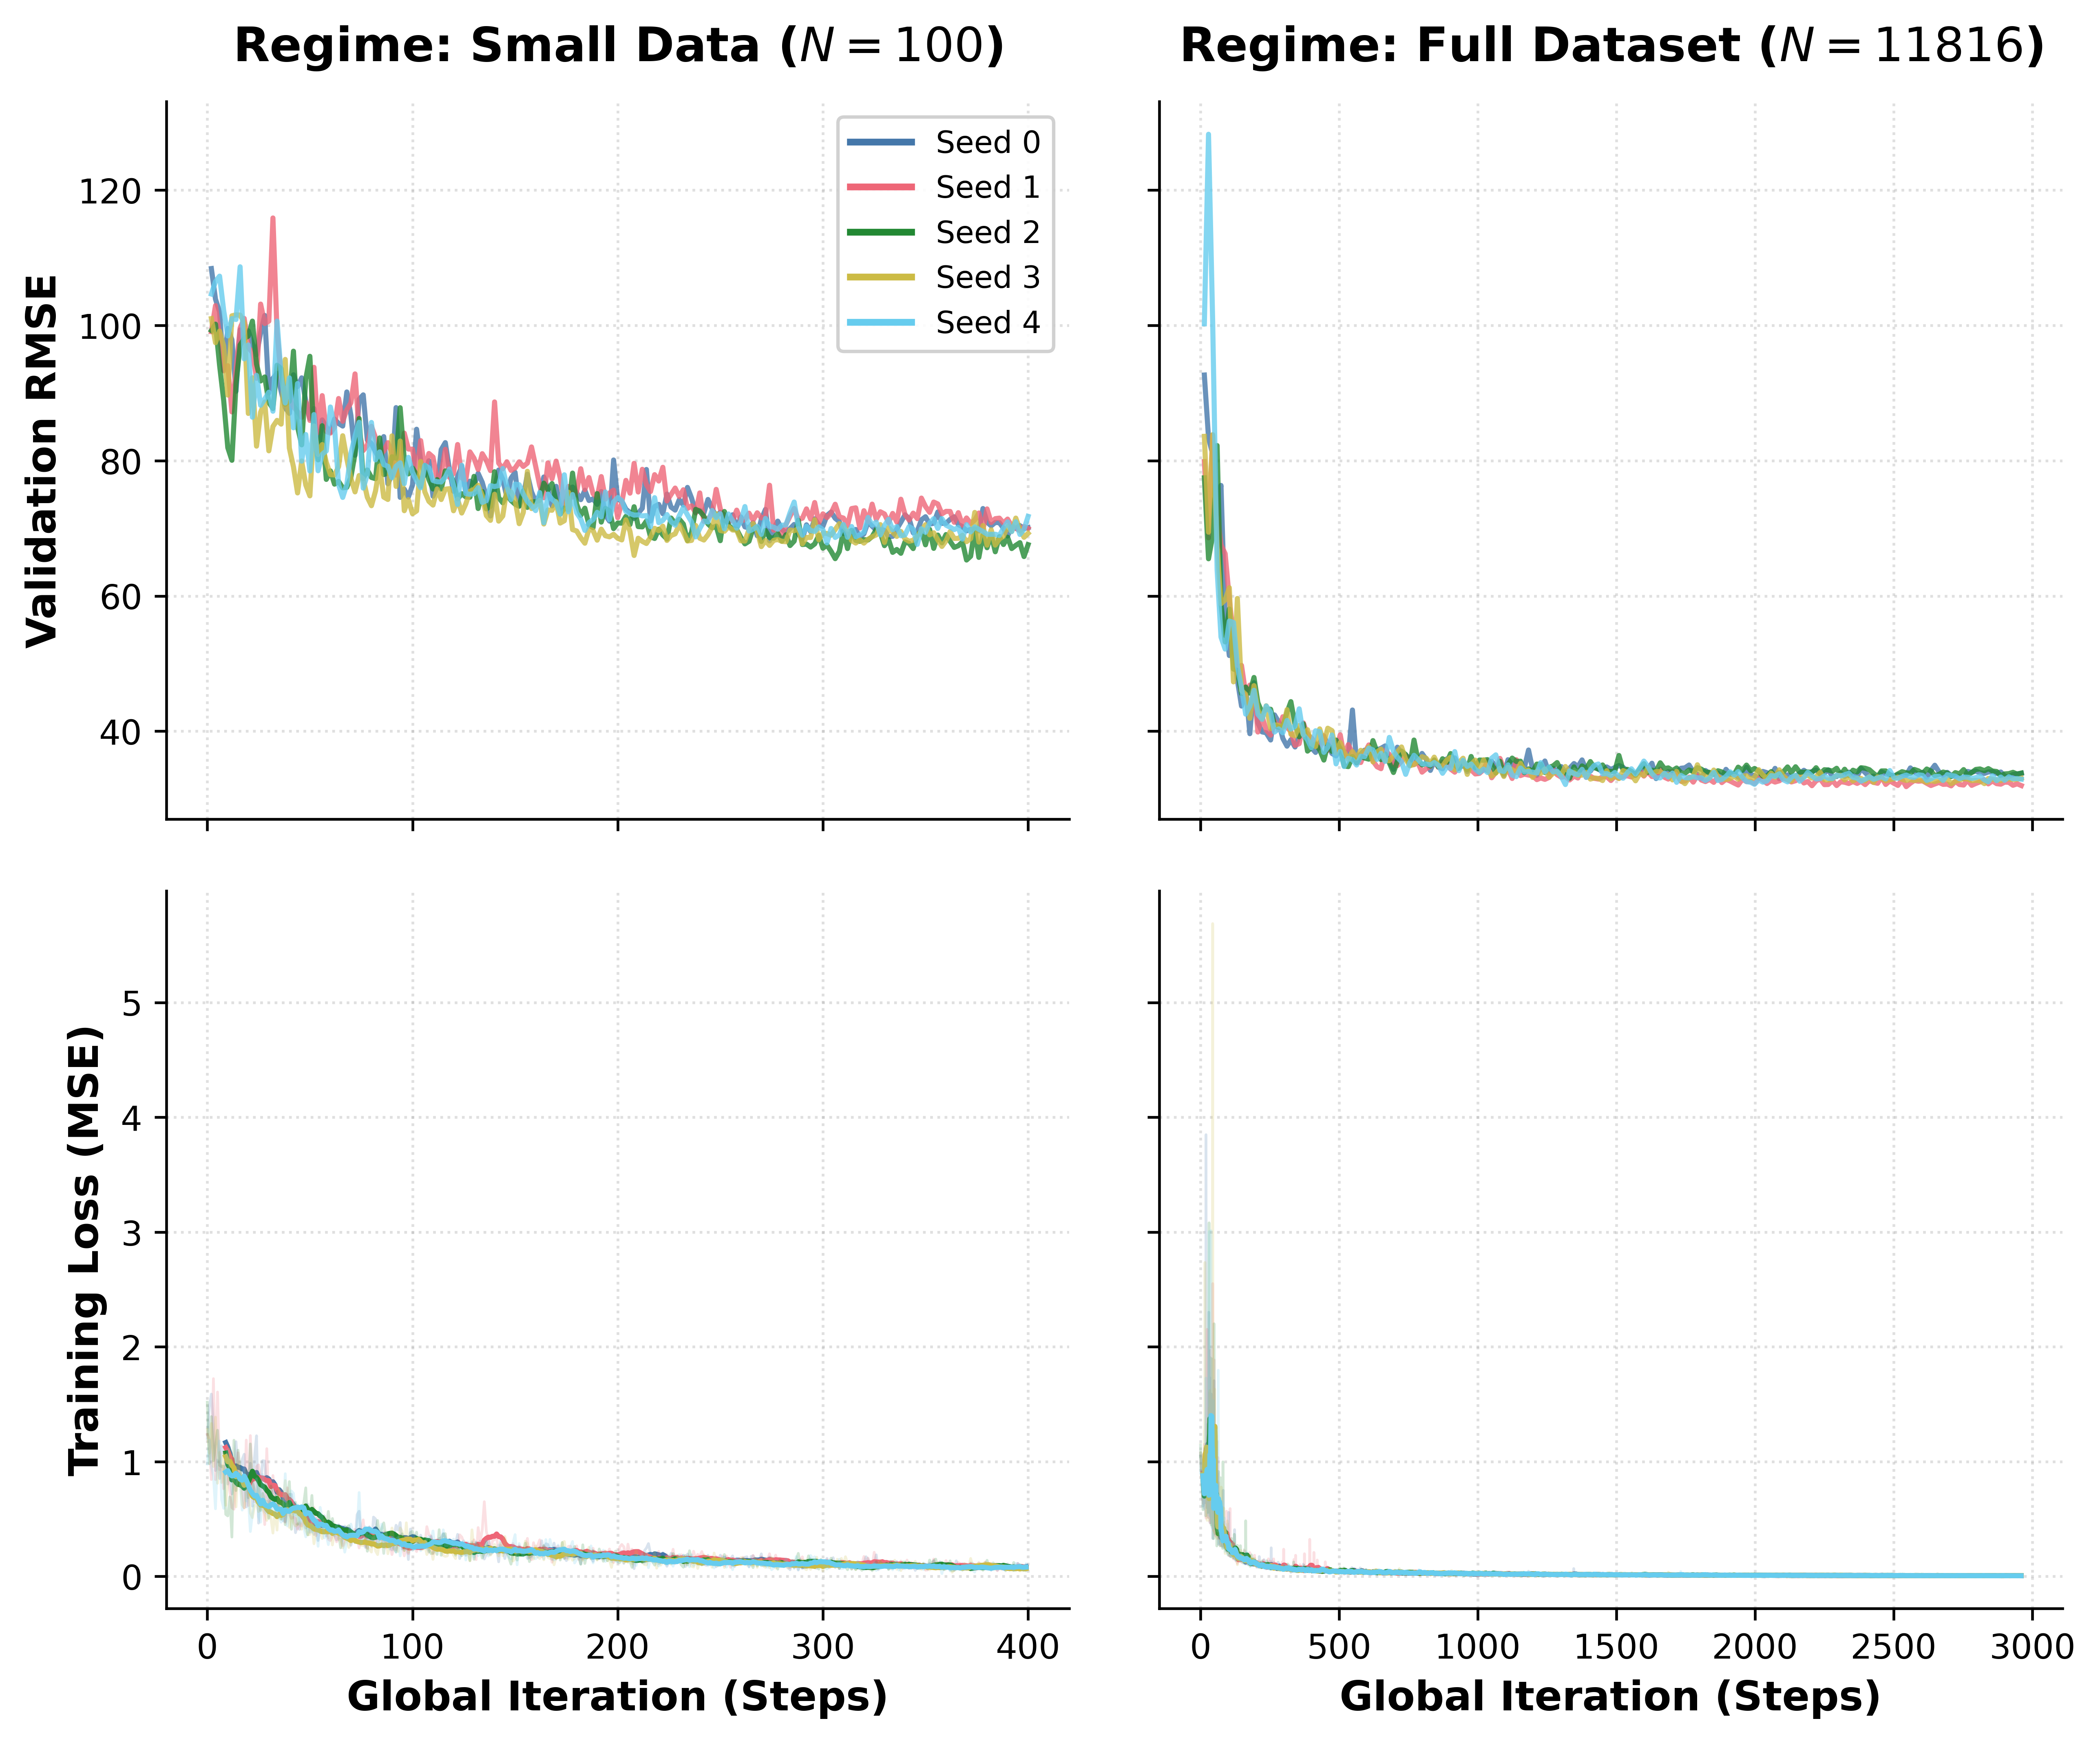
\includegraphics[width=0.8\linewidth]{figures/si_convergence_comparison.png}
    \caption{\textbf{Training and validation convergence under fixed training horizons.}
    Validation RMSE (top) and training MSE (bottom) across five random seeds for the Deep4Chem dataset in a small-data regime ($N = 100$, left) and the full dataset ($N = 11{,}816$, right). Using a fixed y-axis for direct comparison, the plots show rapid stabilization for large $N$ and expected stochasticity for small $N$. The absence of late-epoch divergence in either regime supports the use of a fixed training horizon for cross-model comparisons.
    }
    \label{fig:si-convergence}
\end{figure}
\section{Variance Component Estimation}
\label{si:variance_derivation}

\subsection{Model Specification}
To quantify the sources of predictive variability, we employ a fully nested ANOVA design. Let $y_{ijk}$ denote the performance metric (RMSE) for the $k$-th replicate of the $j$-th regression head trained on the $i$-th encoder. The experimental design consists of 125 independent training runs structured as follows:
\begin{itemize}
    \item $i = 1, \dots, a$: Number of independent Encoder training runs ($a=5$).
    \item $j = 1, \dots, b$: Number of independent Head training runs nested within each encoder ($b=5$).
    \item $k = 1, \dots, n$: Number of independent random seed replicates per head ($n=5$).
\end{itemize}

The statistical model is:
\begin{equation}
y_{ijk} = \mu + A_i + B_{j(i)} + \varepsilon_{ijk}
\end{equation}
where:
\begin{itemize}
    \item $\mu$ is the grand mean.
    \item $A_i \sim \mathcal{N}(0, \sigma_A^2)$ is the random effect of the \textbf{Encoder}.
    \item $B_{j(i)} \sim \mathcal{N}(0, \sigma_{B|A}^2)$ is the random effect of the \textbf{Head} (nested within Encoder).
    \item $\varepsilon_{ijk} \sim \mathcal{N}(0, \sigma_\varepsilon^2)$ is the residual error (seed variability).
\end{itemize}

\subsection{Sum of Squares and Mean Squares}
We compute the Sum of Squares (SS) and Mean Squares (MS) as follows:

\paragraph{1. Encoders (Factor A)}
\begin{align}
SS_A &= b n \sum_{i=1}^{a} (\bar{y}_{i..} - \bar{y}_{...})^2 \\
MS_A &= \frac{SS_A}{a - 1}
\end{align}

\paragraph{2. Heads within Encoders (Factor B nested in A)}
\begin{align}
SS_{B(A)} &= n \sum_{i=1}^{a} \sum_{j=1}^{b} (\bar{y}_{ij.} - \bar{y}_{i..})^2 \\
MS_{B(A)} &= \frac{SS_{B(A)}}{a(b - 1)}
\end{align}

\paragraph{3. Residual / Error}
\begin{align}
SS_E &= \sum_{i=1}^{a} \sum_{j=1}^{b} \sum_{k=1}^{n} (y_{ijk} - \bar{y}_{ij.})^2 \\
MS_E &= \frac{SS_E}{ab(n - 1)}
\end{align}

\subsection{Expected Mean Squares (EMS) and Estimators}
Assuming a balanced design and random effects, the Expected Mean Squares are:
\begin{align}
\mathbb{E}[MS_A] &= \sigma_\varepsilon^2 + n \sigma_{B|A}^2 + bn \sigma_A^2 \\
\mathbb{E}[MS_{B(A)}] &= \sigma_\varepsilon^2 + n \sigma_{B|A}^2 \\
\mathbb{E}[MS_E] &= \sigma_\varepsilon^2
\end{align}

By solving this system of linear equations, we obtain the Method of Moments estimators used in the main text:
\begin{align}
\hat{\sigma}_\varepsilon^2 &= MS_E \\
\hat{\sigma}_{B|A}^2 &= \frac{MS_{B(A)} - MS_E}{n} \\
\hat{\sigma}_A^2 &= \frac{MS_A - MS_{B(A)}}{bn}
\end{align}
In cases where an estimate is negative it is clamped to zero.

\subsection{Bootstrap Uncertainty Analysis}
\begin{table}[ht]
\centering
\caption{Bootstrap confidence intervals for variance component proportions. Mean estimates and 95\% bootstrap confidence intervals for the proportion of total predictive variance attributable to encoder stochasticity (A), head stochasticity (B(A)), and residual seed noise (E) across training set sizes on the Deep4Chem dataset. Variance components were estimated using the ANOVA Method of Moments under a balanced nested design ($I=5$, $J=5$, $K=5$). Due to the limited number of encoders and heads, confidence intervals are wide, particularly in low-data regimes; estimates should therefore be interpreted qualitatively.}
\label{tab:si_varcomp_bootstrap}
\begin{tabular}{lccccccccc}
\toprule
\textbf{Subset} &
\multicolumn{3}{c}{\textbf{Encoders (A)}} &
\multicolumn{3}{c}{\textbf{Heads (B(A))}} &
\multicolumn{3}{c}{\textbf{Residual (E)}} \\
\cmidrule(lr){2-4} \cmidrule(lr){5-7} \cmidrule(lr){8-10}
 & Mean & CI$_{low}$ & CI$_{high}$
 & Mean & CI$_{low}$ & CI$_{high}$
 & Mean & CI$_{low}$ & CI$_{high}$ \\
\midrule
N00050  & 0.646 & 0.028 & 0.853 & 0.182 & 0.022 & 0.731 & 0.172 & 0.058 & 0.459 \\
N00100  & 0.765 & 0.184 & 0.894 & 0.100 & 0.031 & 0.561 & 0.134 & 0.049 & 0.335 \\
N00250  & 0.603 & 0.000 & 0.791 & 0.195 & 0.082 & 0.691 & 0.202 & 0.068 & 0.536 \\
N01000  & 0.943 & 0.083 & 0.977 & 0.042 & 0.015 & 0.619 & 0.015 & 0.003 & 0.369 \\
N11816  & 0.917 & 0.516 & 0.960 & 0.029 & 0.007 & 0.226 & 0.054 & 0.021 & 0.274 \\
\bottomrule
\end{tabular}
\end{table}

\paragraph{Bootstrap uncertainty analysis.}
To assess the robustness of the variance component estimates, we performed a nonparametric bootstrap by resampling encoder--head--replicate triplets and recomputing variance components for each resample. As shown in Table~\ref{tab:si_varcomp_bootstrap}, confidence intervals are wide in low-data regimes, reflecting the limited number of encoders and heads available for estimation. Nevertheless, across all dataset sizes, the qualitative ordering of variance sources is preserved, with encoder-level stochasticity consistently contributing the largest share of predictive variability.

\section{Head Sensitivity and Fixed-Encoder Ablations}
As shown in Figure~\ref{fig:fixed-model}, holding the encoder fixed isolates variability attributable solely to the regression head. We observe differences in both average performance and variability across heads, with the dashed line marking the end-to-end D-MPNN reference.

\subsection{Fixed-Encoder Head Comparison}
In Figure~\ref{fig:fixed-model}, we fix a trained D-MPNN encoder and evaluate different regression heads, reporting mean performance over 30 seeds with standard deviation. This isolates the contribution of the downstream mapping from the learned representation. Tree-based models, particularly XGBoost, exhibit improved stability and competitive performance relative to neural heads, motivating their use in the hybrid framework.
\begin{figure}[ht]
  \centering
  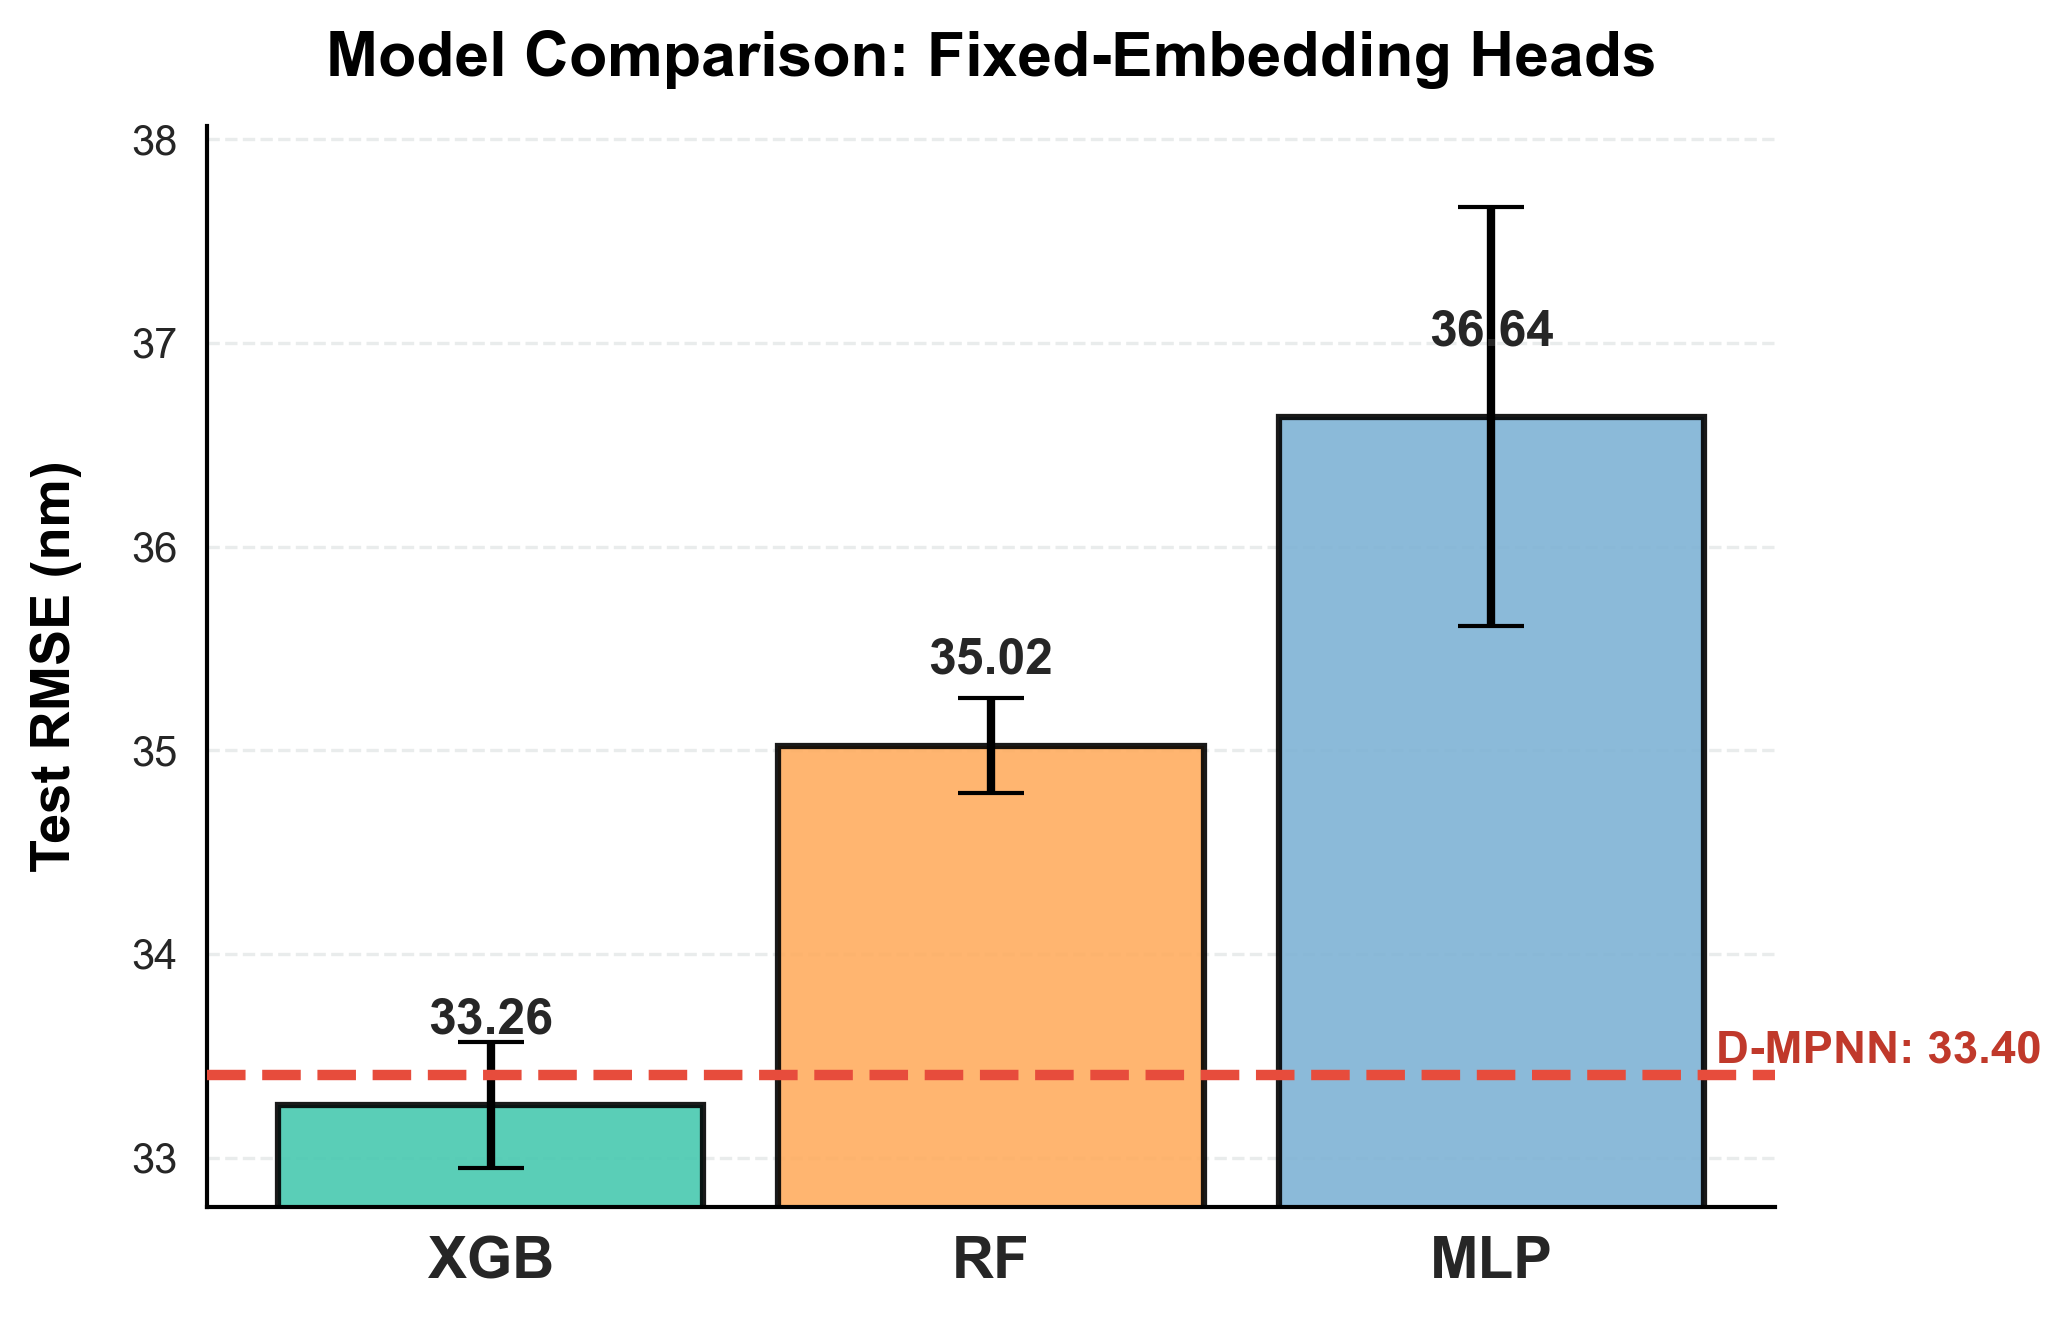
\includegraphics[width=0.9\linewidth]{figures/fixed-encoder-model-comparison.png}
  \caption{\textbf{Test-set RMSE for different regression heads trained on a fixed D-MPNN encoder representation.} Values are the mean $\pm$ SD over 30 seeds. The dashed line represents the performance of the end-to-end D-MPNN model.}
  \label{fig:fixed-model}
\end{figure}

\subsection{Ensembling Effects Across Regimes}
\begin{figure}[ht]
  \centering
  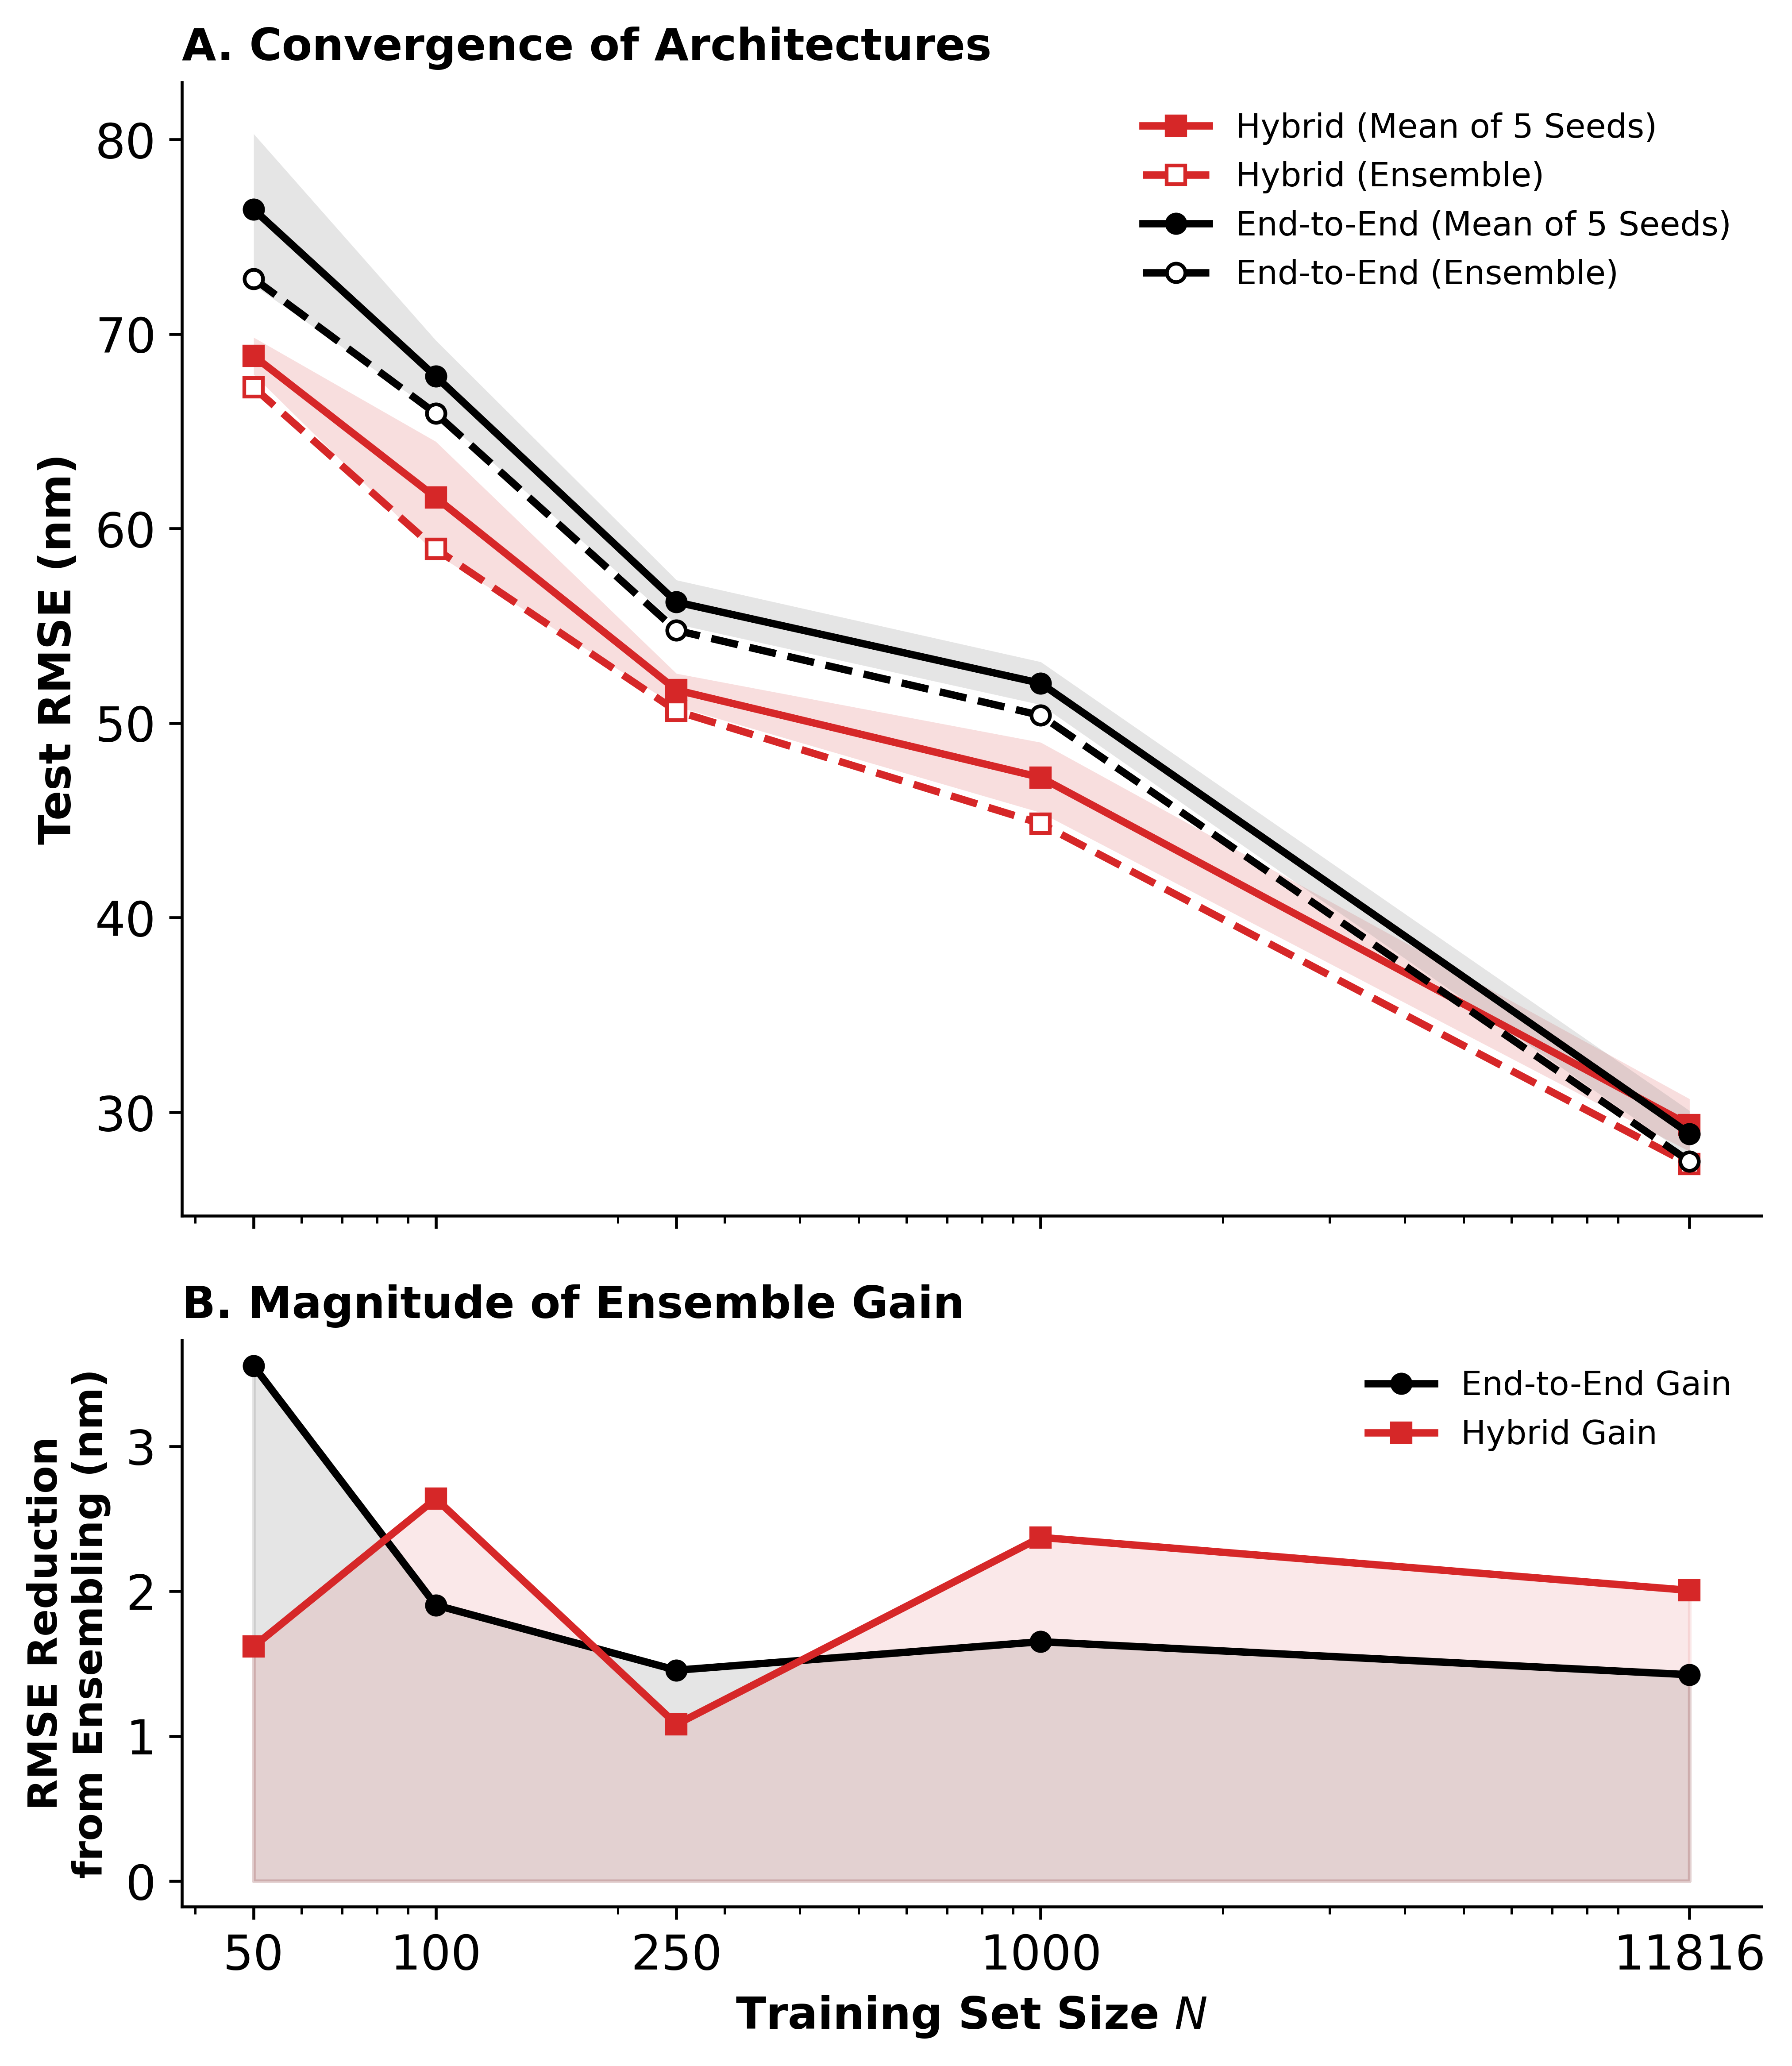
\includegraphics[width=0.6\linewidth]{figures/si_ensemble_split_panel_final.png}
\caption{\textbf{Stability and ensemble analysis.}
Test RMSE on Deep4Chem across training set sizes for the Hybrid (red) and End-to-End (black/gray) models. Solid lines show the mean of five independent training seeds (error bars: one standard deviation), while dashed lines indicate 5-member ensembles.}
  \label{fig:ensemble-vs-n}
\end{figure}

\paragraph{Ensembling effects and stability across regimes.}
Figure~\ref{fig:ensemble-vs-n} compares individual models to ensemble predictions obtained by averaging independently trained instances. Ensembling consistently reduces test-set RMSE for both hybrid and end-to-end models, with the largest gains observed in low-data regimes. The improvement is most pronounced where performance is most variable, indicating that averaging helps mitigate run-to-run instability. 

This pattern is consistent with the variance decomposition results. In low-data settings ($N \leq 250$), predictive performance is limited by both variability in the learned representation and sensitivity of the downstream mapping. The hybrid model primarily reduces the latter, while ensembling further improves performance by averaging over variability in the representation.

\paragraph{Implications of Ensemble Performance on Representation Diversity.} 
Ensemble theory shows that averaging predictions reduces error when individual models make partially uncorrelated mistakes~\cite{Krogh1995}. The performance gains observed for the hybrid ensemble relative to individual D-MPNNs therefore suggest that the models capture different aspects of the chemical space, leading to prediction errors that are not fully correlated.

\section{Emission Prediction and Physical Limitations}

To assess generalization, we extend our analysis to peak emission wavelength prediction. This task is more challenging than absorption prediction, as emission depends on excited-state relaxation and solvent reorganization (Stokes shift), which are not captured by the ground-state molecular graphs used as input.

Figure~\ref{fig:em-multipanel-n-vs-rmse} shows test RMSE for emission prediction under scaffold splits. Unlike absorption, where the hybrid advantage is consistent, emission exhibits a regime-dependent trade-off. In the Deep4Chem and DSSCDB datasets, hybrid and end-to-end models perform similarly, with the end-to-end model showing a slight advantage at larger $N$.

In ChemFluor, performance varies more across $N$, and neither architecture shows a consistent advantage over the full range. Overall, these results suggest that hybridization is most effective when the learned representation captures the dominant drivers of the target property. For emission, additional excited-state and solvent reorganization effects are likely not captured by the current inputs, and may require either richer features or end-to-end adaptation.

\begin{figure}[ht]
  \centering
  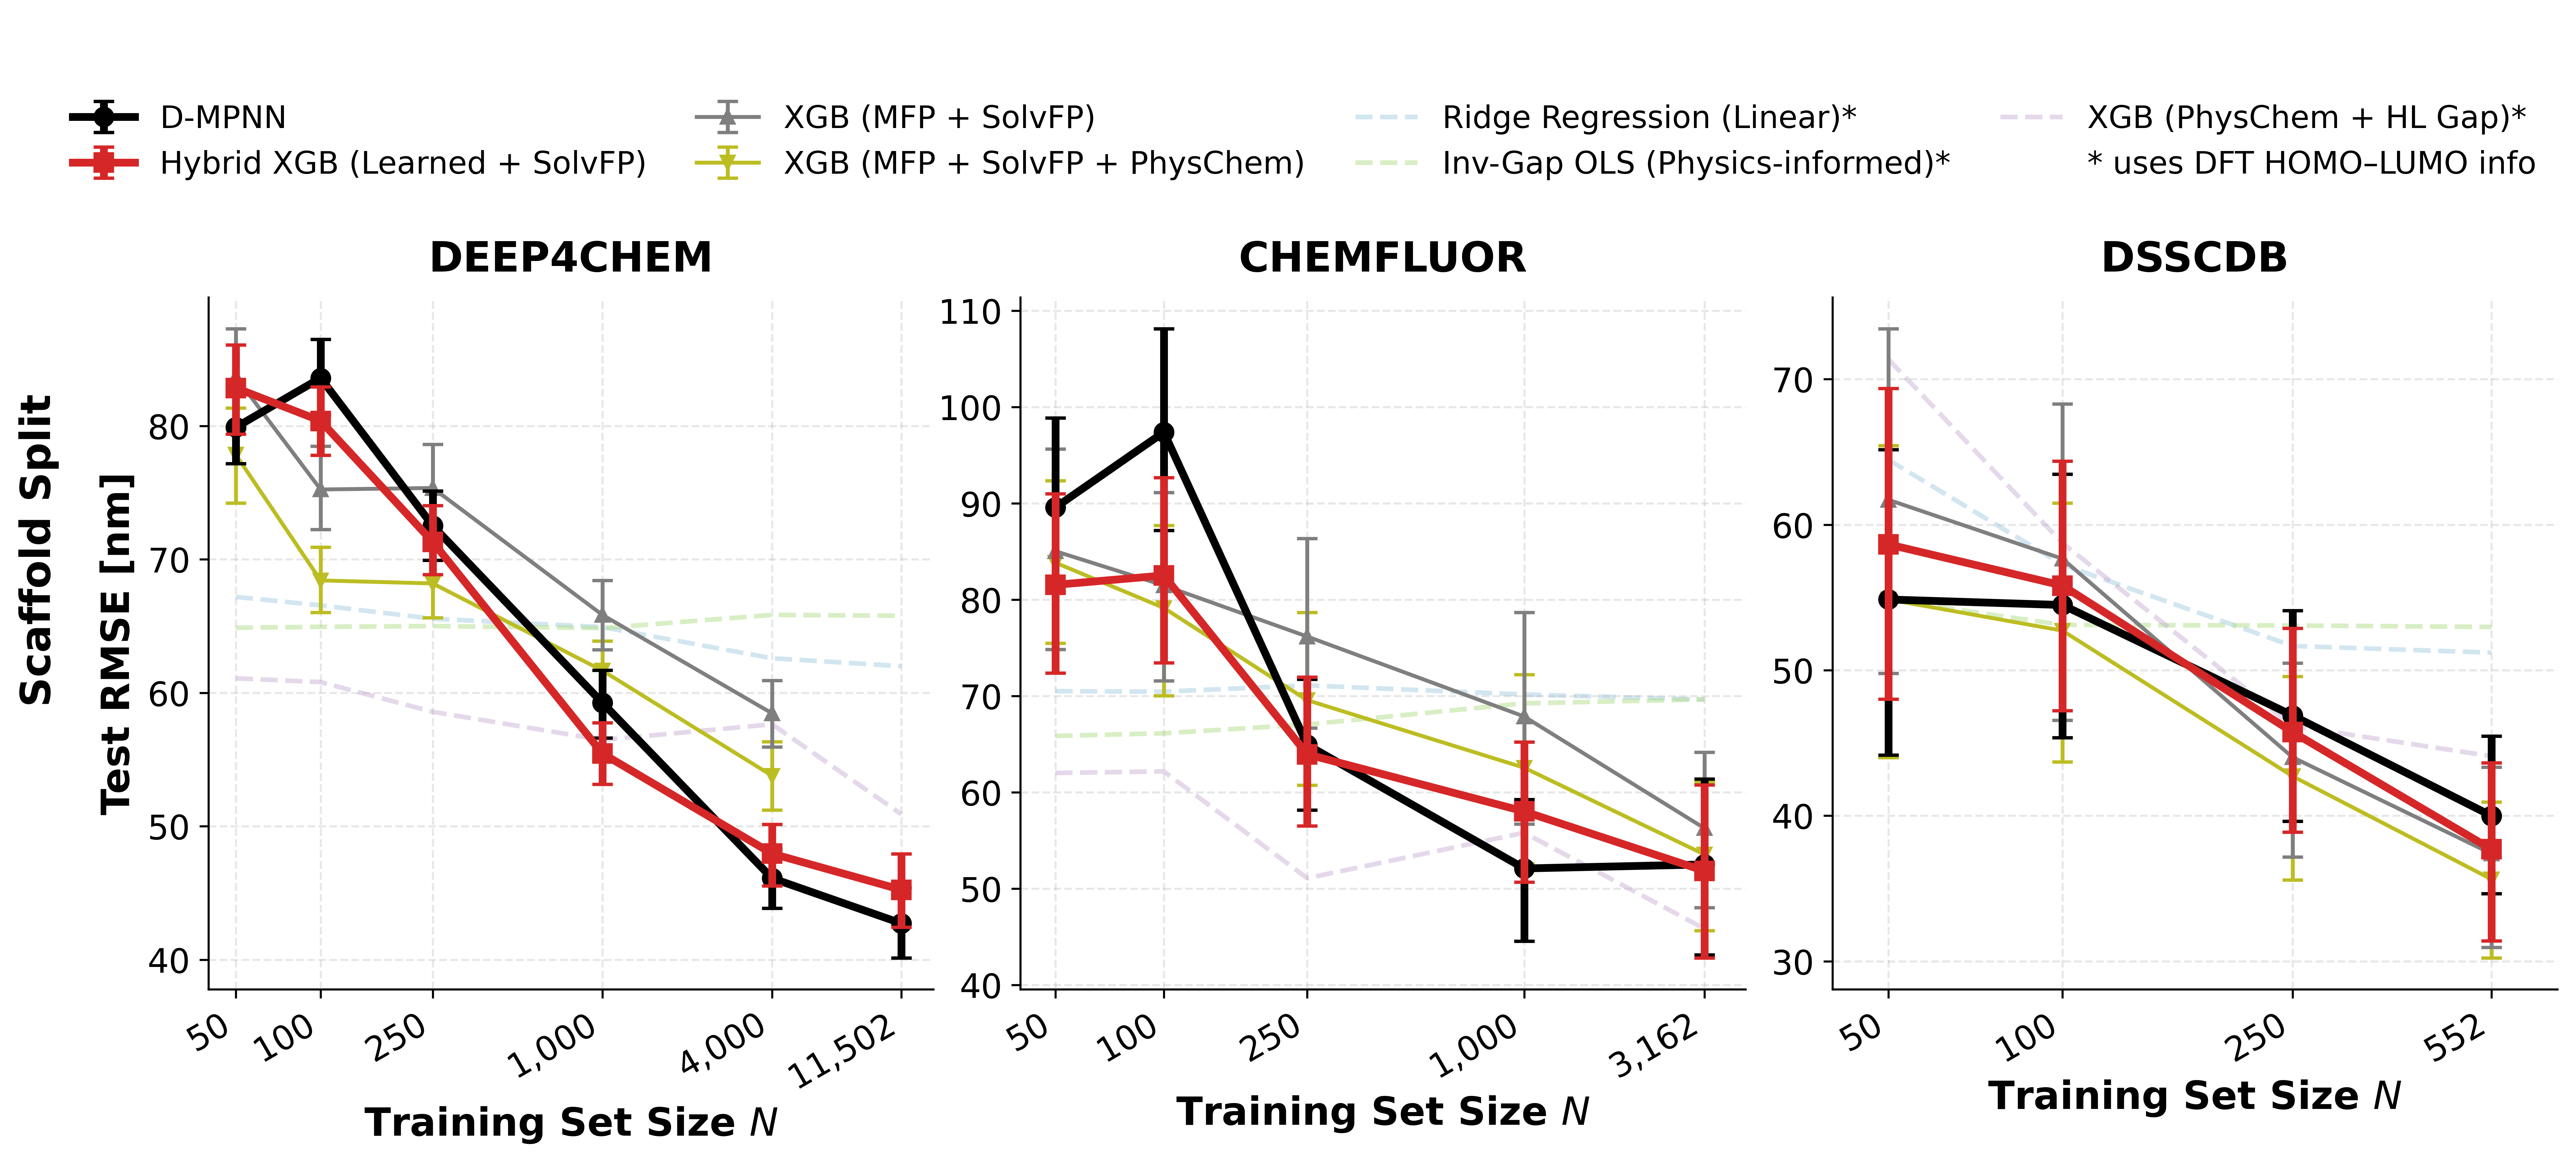
\includegraphics[width=0.9\linewidth]{figures/em_multipanel_bootstrap_ci.png}
  \caption{\textbf{Peak emission wavelength prediction across Deep4Chem, DSSCDB, and ChemFluor.} Test RMSE versus training set size $N$ (scaffold split). Each panel uses the dataset-specific $N$ values. Error bars indicate 95\% bootstrap confidence intervals for the test RMSE, computed by resampling test molecules with replacement (2000 replicates).}
  \label{fig:em-multipanel-n-vs-rmse}
\end{figure}

\section{Latent Representations}

\subsection{Cross-Seed Stability of Principal Components}
Table~\ref{tab:pc0_stability_deep4chem} shows that the dominant latent component ($PC_0$) exhibits highly consistent correlations with both the HOMO--LUMO gap and the target absorption wavelength across independently trained encoder seeds.
\begin{table}[ht]
\centering
\caption{Cross-seed stability of correlations between the dominant latent component (PC$_0$) and key physical properties on the Deep4Chem dataset. Values represent the Spearman correlation coefficient ($\rho$) for each independently trained encoder seed.}
\label{tab:pc0_stability_deep4chem}
\begin{tabular}{lcc}
\toprule
Encoder Seed & \textbf{PC$_0$ vs.\ HOMO--LUMO Gap} & \textbf{PC$_0$ vs.\ $\lambda_{\max}$} \\
\midrule
0 & $-0.817$ & $0.942$ \\
1 & $-0.819$ & $0.941$ \\
2 & $-0.826$ & $0.941$ \\
3 & $-0.811$ & $0.939$ \\
4 & $-0.827$ & $0.947$ \\
\midrule
\textbf{Aggregate} & $\mathbf{-0.820 \pm 0.007}$ & $\mathbf{0.942 \pm 0.003}$ \\
\bottomrule
\end{tabular}
\end{table}

\FloatBarrier

\subsection{Interpretation of Higher-Order Principal Components}

While the dominant principal components admit relatively clear chemical interpretations, several higher-order dimensions exhibit weaker or more diffuse correlations with the selected descriptor set. Below, we summarize the most prominent trends visible in Figure~\ref{fig:pc-physchem-heatmap} of the main text, noting that these interpretations are necessarily tentative.

\paragraph{$PC_3$: Weak Size and Flexibility Signal.}
Unlike $PC_2$, which captures global molecular size in a coherent manner, $PC_3$ displays comparatively weak negative correlations with \textit{NumRotatableBonds} ($\rho = -0.29$), \textit{ExactMolWt} ($\rho = -0.19$), and \textit{HeavyAtomCount} ($\rho = -0.19$). These magnitudes suggest only a mild association with molecular compactness or flexibility, and do not support a strong one-dimensional physical interpretation.

\paragraph{$PC_4$ and $PC_5$: Low-Amplitude Structural Variation.}
Both $PC_4$ and $PC_5$ exhibit generally weak correlations ($|\rho| < 0.3$) across the descriptor panel. $PC_5$ shows a modest negative association with \textit{FractionCSP3} ($\rho = -0.29$), while $PC_4$ lacks a dominant alignment with any individual descriptor. These components likely reflect distributed structural effects or composite interactions rather than a single chemically interpretable axis.

\paragraph{$PC_6$: Hybridization Sensitivity.}
$PC_6$ shows a moderate negative correlation with \textit{FractionCSP3} ($\rho = -0.33$), indicating sensitivity to the degree of sp$^3$ character. This pattern is consistent with a distinction between more planar, conjugated systems and more saturated, three-dimensional scaffolds, though the effect size remains secondary relative to the dominant axes.

\paragraph{$PC_7$: Polarity-Associated Variation.}
$PC_7$ exhibits moderate negative correlations with \textit{TPSA} ($\rho = -0.33$) and \textit{NumHBA} ($\rho = -0.29$), alongside smaller associations with flexibility-related descriptors. This suggests sensitivity to polarity-related substitution patterns, though again without a uniquely defining descriptor signature.

\paragraph{$PC_9$ and Higher Components: Diffuse Effects.}
Higher-order components such as $PC_9$ show no strong monotonic correlations with the evaluated descriptors ($|\rho| \le 0.16$). Nevertheless, some of these dimensions are ranked as moderately important by the downstream XGBoost model. This is consistent with the fact that PCA is a linear projection applied to a highly nonlinear learned representation; individual components need not correspond to simple, one-dimensional chemical quantities. Instead, these higher-order directions likely encode nonlinear interactions, composite structural motifs, or dataset-specific variation not captured by standard descriptor panels.


\subsection{ChemFluor Correlation Map}
Having established that the dominant principal component is stable across encoder seeds for Deep4Chem, here we examine whether similar structure emerges on the ChemFluor dataset.
\begin{figure*}[ht]
 \centering
 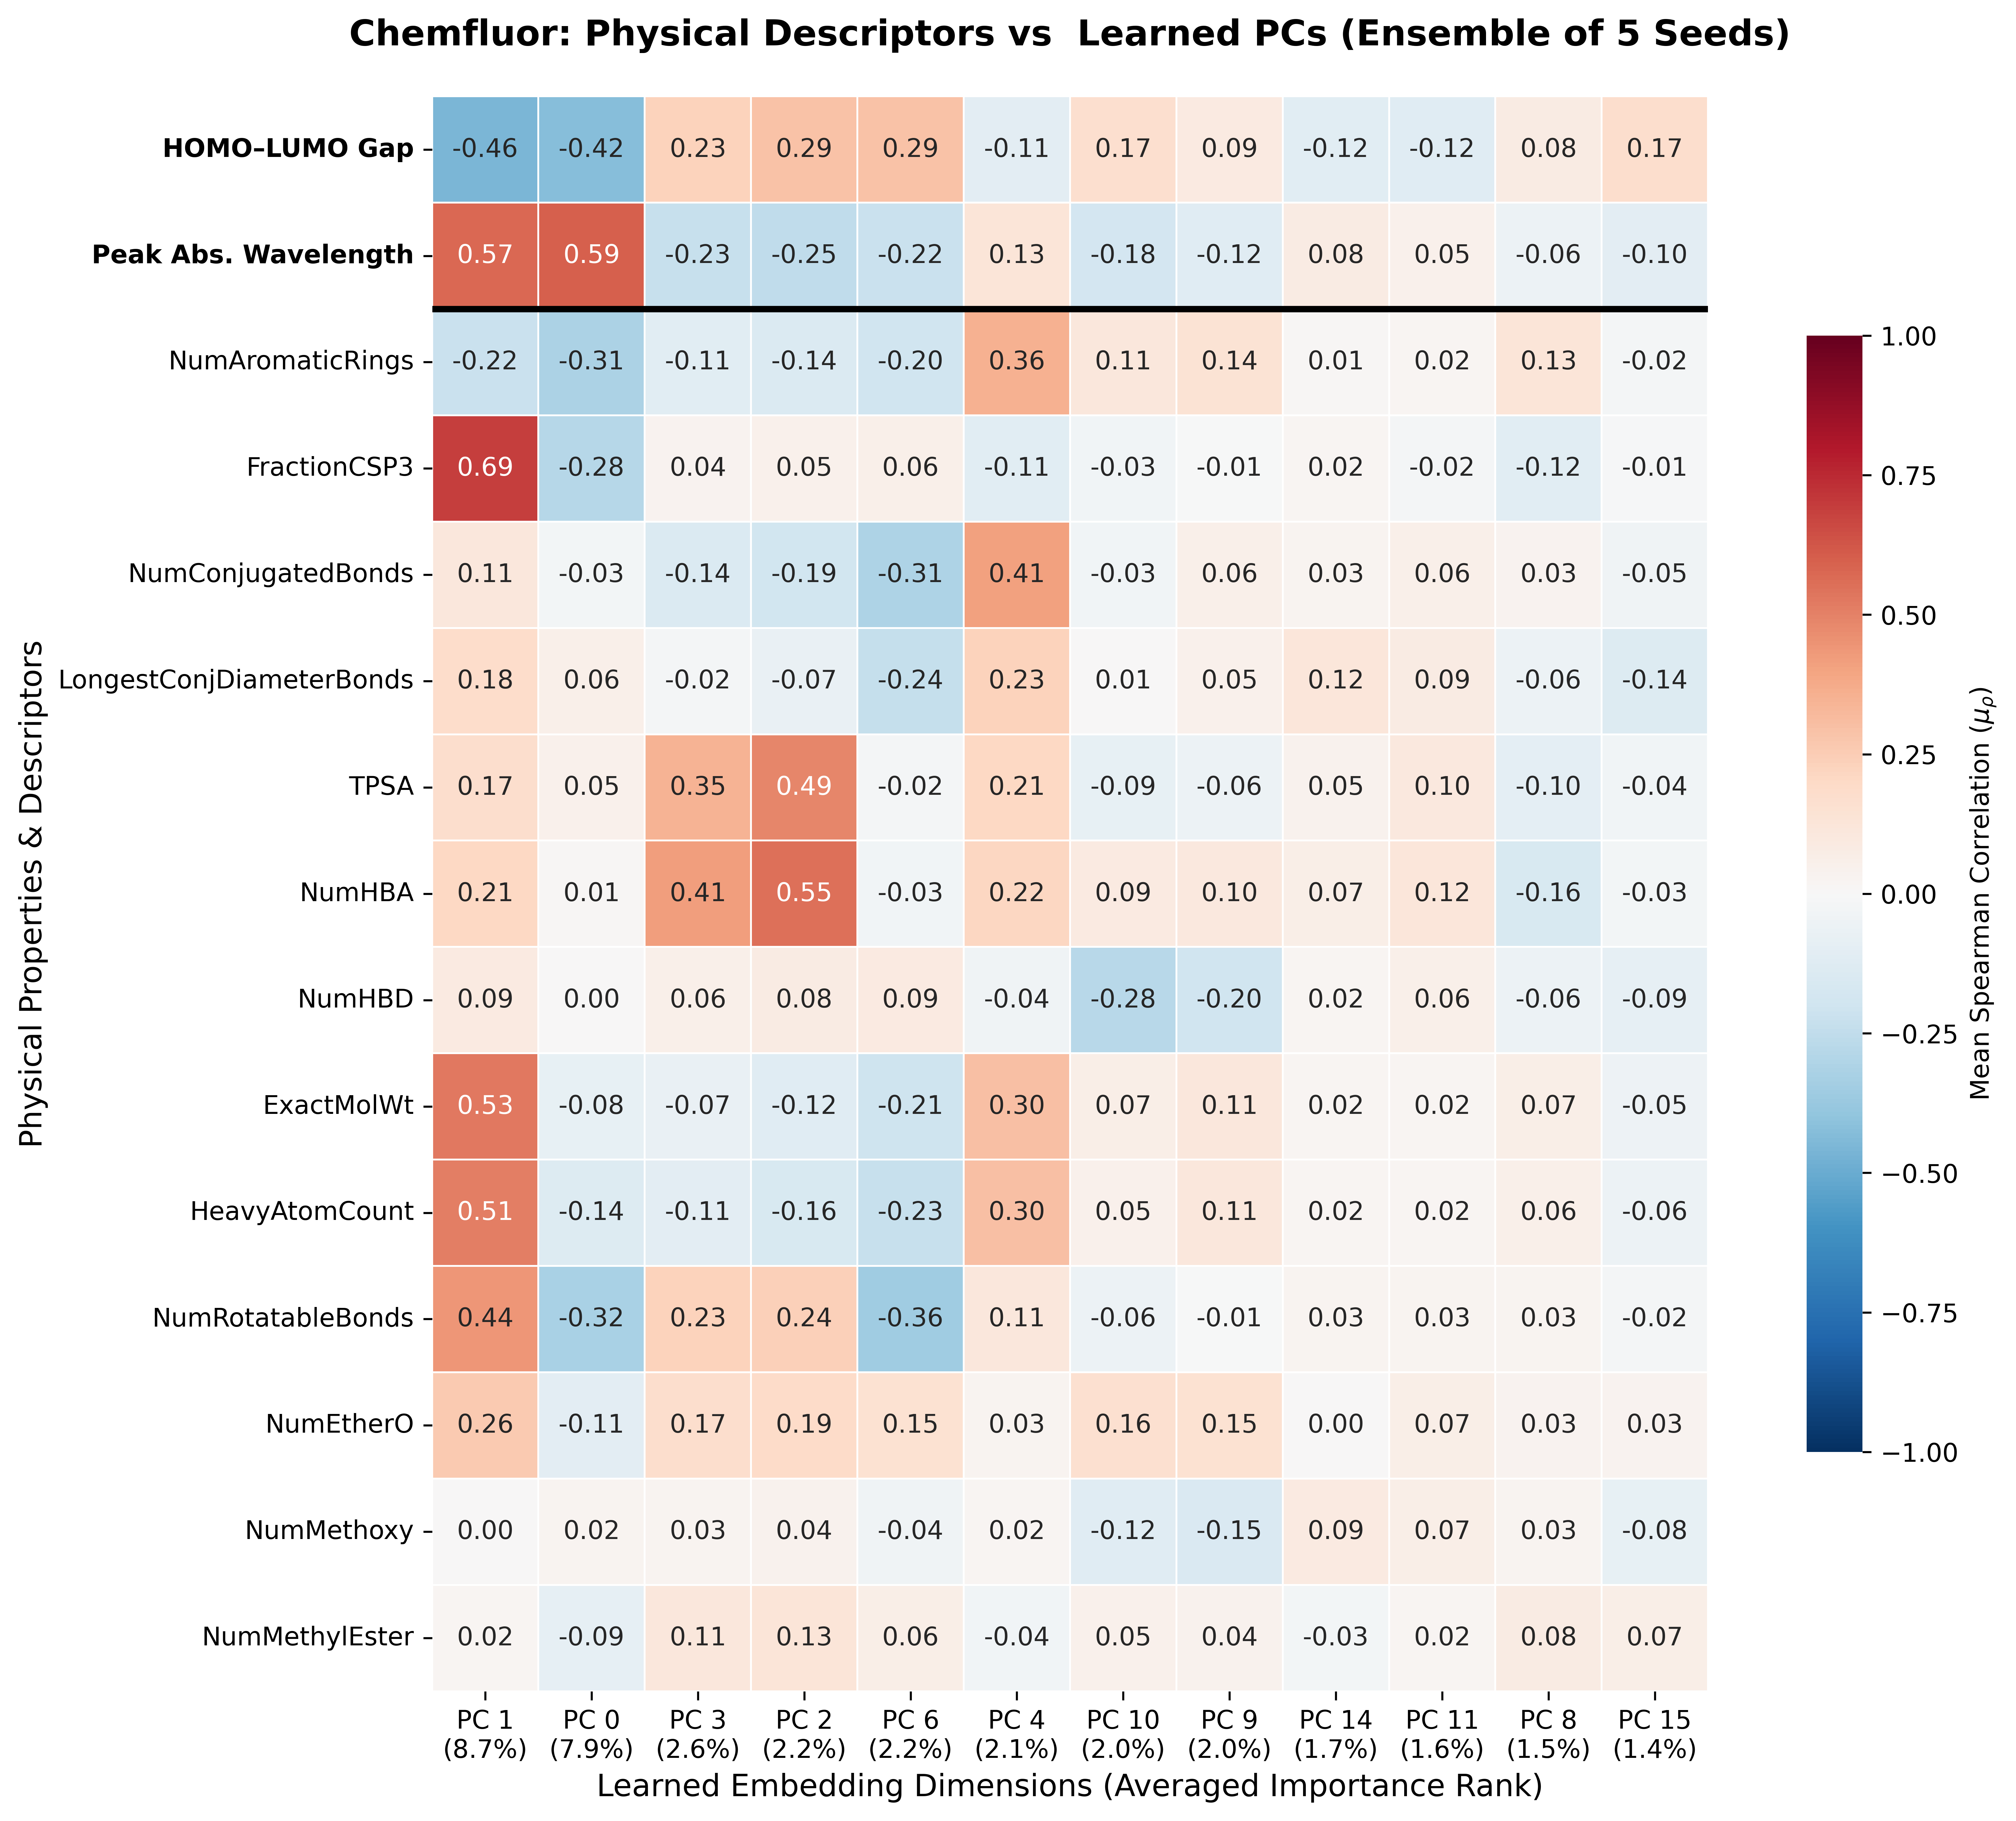
\includegraphics[width=0.75\textwidth]{figures/chemfluor-pc-physchem-heatmap.png}
\caption{\textbf{Consensus Interpretability Map: Learned PCs vs Physics.} 
Aligned Spearman rank correlations between the top 12 predictive principal components (PCs) and physicochemical descriptors across an ensemble of 5 seeds on the ChemFluor dataset. PCs are ordered by averaged XGB feature importance. The horizontal divider separates structural descriptors from the photophysical targets, HOMO--LUMO gap and peak absorption wavelength.}
\label{fig:chemfluor-pc-physchem-heatmap}
\end{figure*}

\FloatBarrier

\subsection{Latent Density Analyses}
Figure~\ref{fig:si_hexbins} presents hexbin density plots illustrating the relationship between selected latent principal components and independent physicochemical descriptors. The top principal components exhibit structured alignment with chemically meaningful axes. In particular, $PC_0$ correlates strongly with effective conjugation length and primary optical targets, $PC_2$ tracks molecular size through molecular weight and heavy atom count, $PC_8$ reflects polarity and hydrogen-bonding capacity, and $PC_1$ captures aromatic core complexity. These relationships support the interpretation that the learned representation organizes molecules along physically meaningful dimensions rather than arbitrary latent directions.
\begin{figure*}[ht]
  \centering
  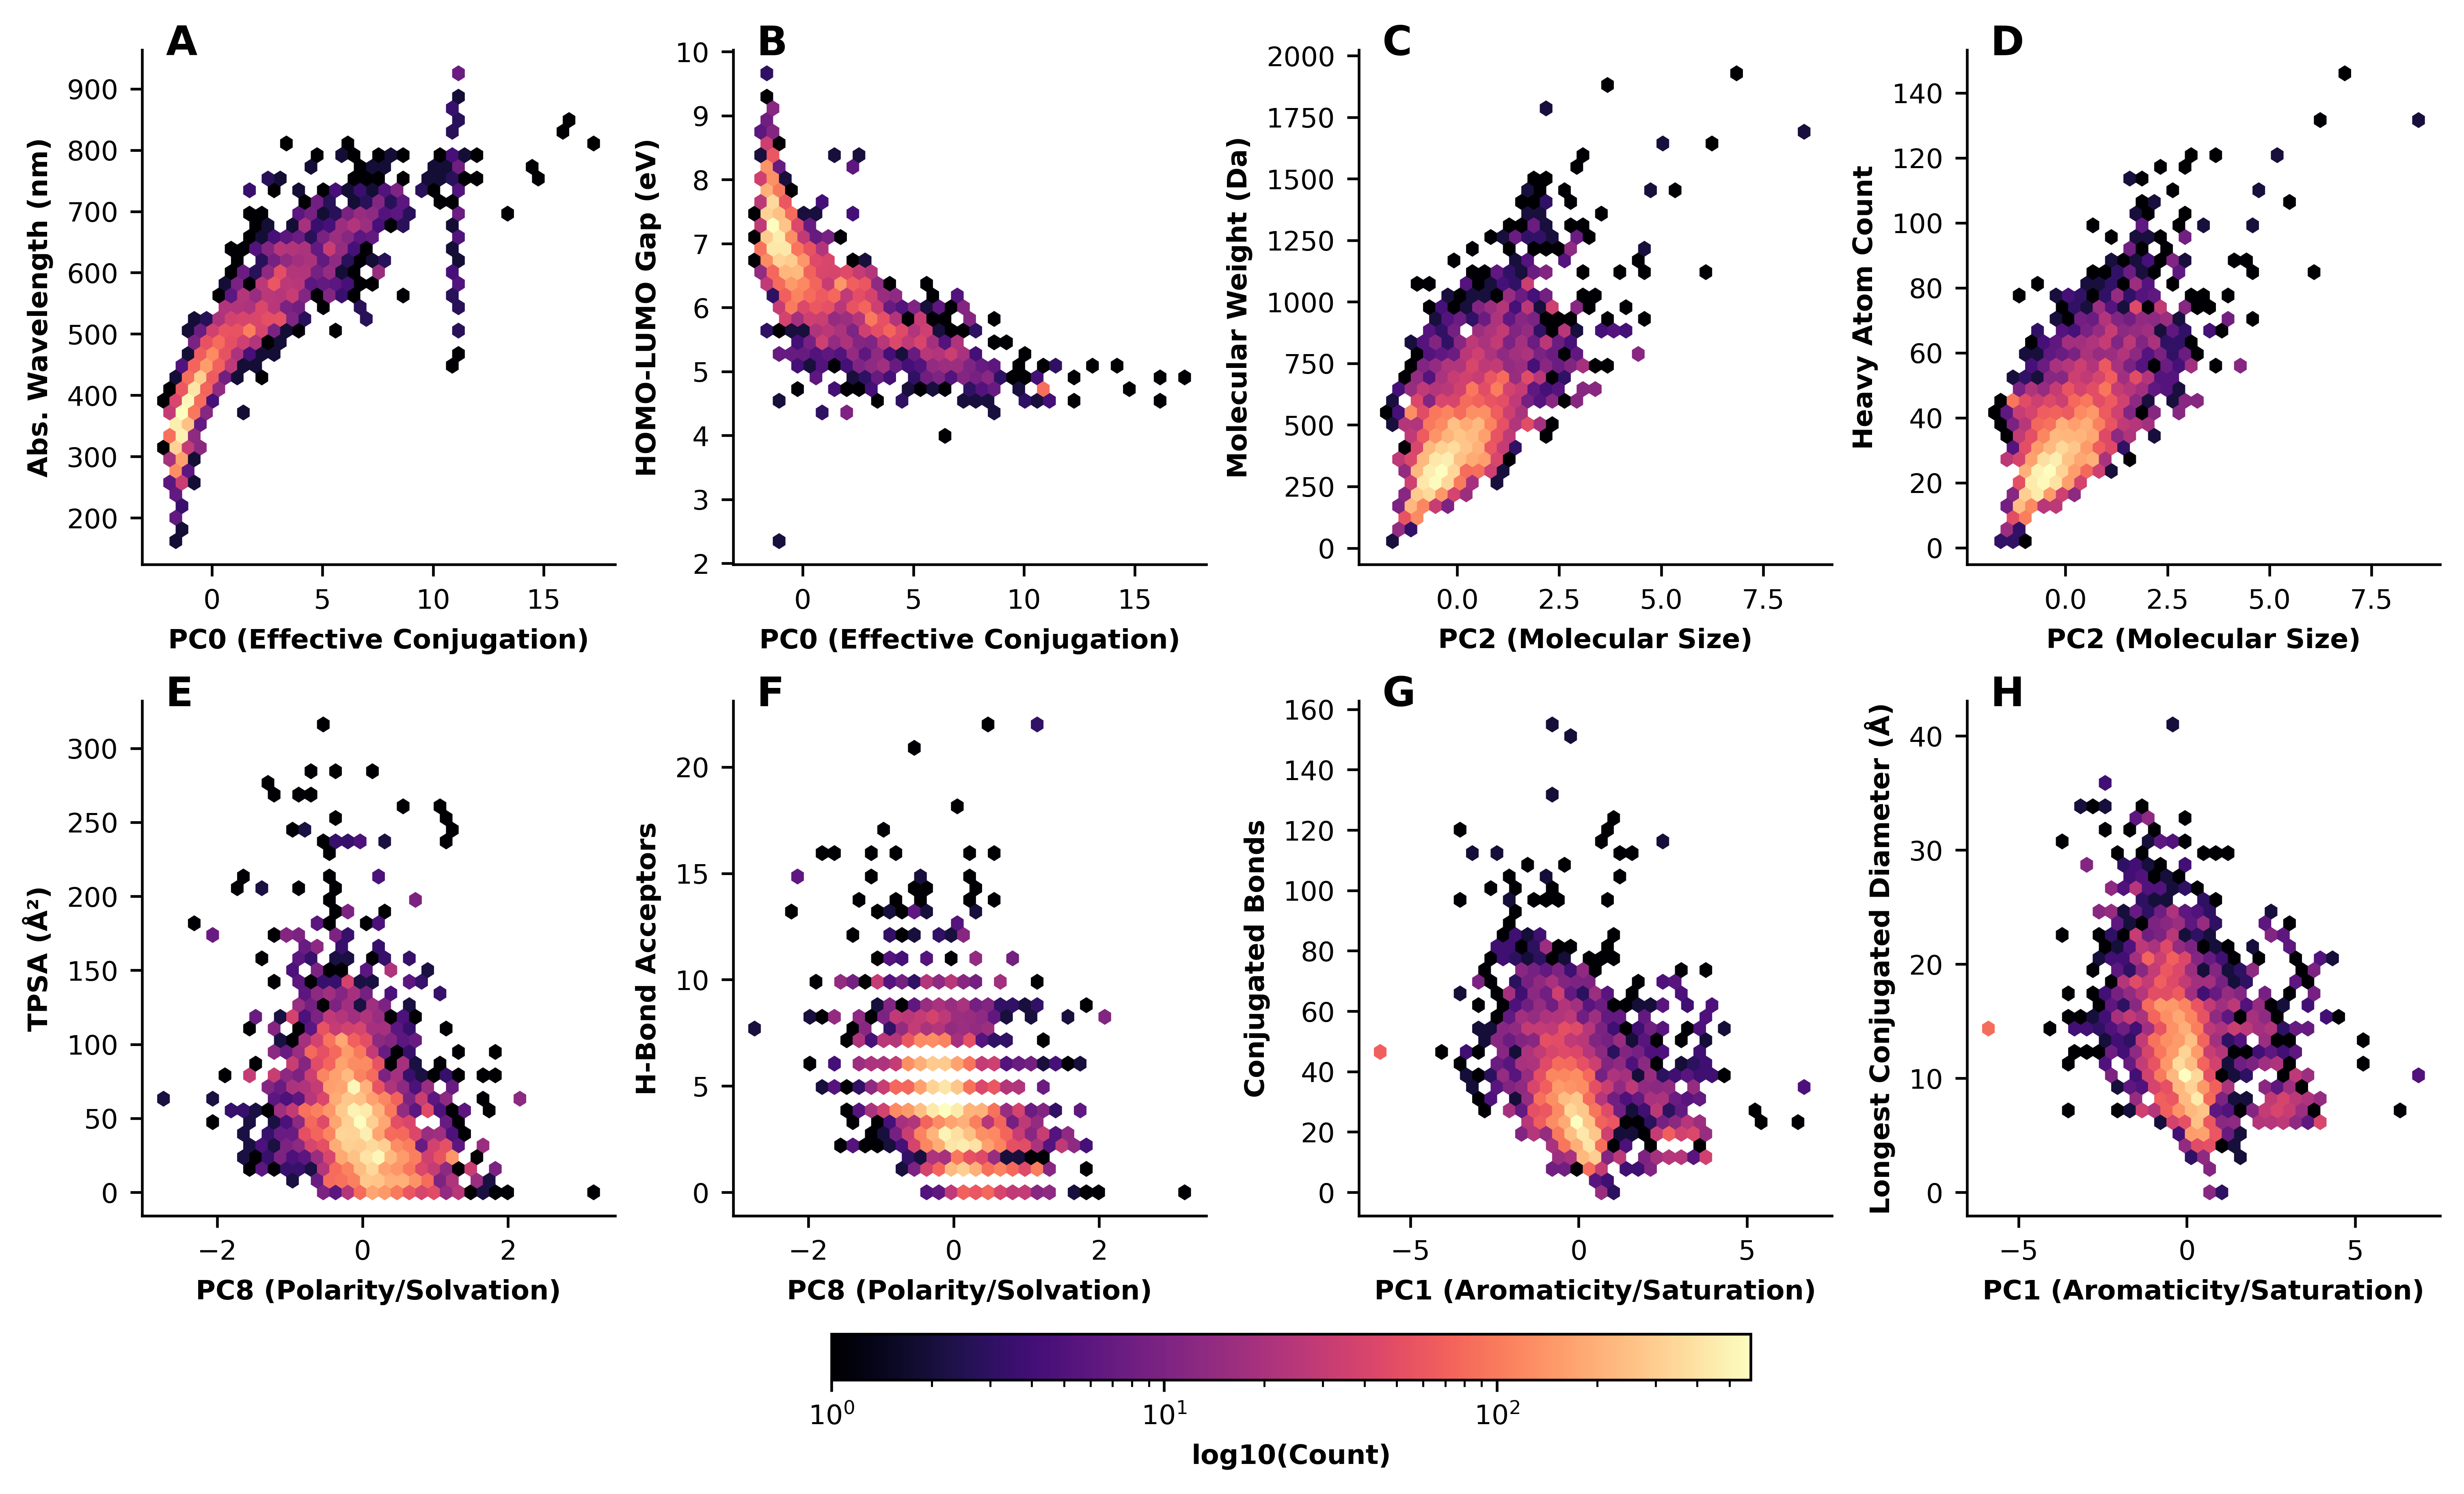
\includegraphics[width=0.8\textwidth]{figures/Figure_SI_Latent_Densities.png}
  \caption{\textbf{Density distribution of latent dimensions against physicochemical descriptors.} Hexbin plots (log-scaled density) demonstrate the alignment of the top Principal Components (PCs) with independent physical properties. 
  \textbf{(A-B)} $PC_0$ captures the effective conjugation length, showing strong correlation with the primary targets. 
  \textbf{(C-D)} $PC_2$ functions as a molecular size axis, tracking weight and heavy atom count. 
  \textbf{(E-F)} $PC_8$ encodes polarity and hydrogen-bonding capacity (TPSA and NumHBA). 
  \textbf{(G-H)} $PC_1$ distinguishes aromatic core complexity, as evidenced by its relationship with conjugated bond count and diameter.}
  \label{fig:si_hexbins}
\end{figure*}

While marginal density plots reveal pairwise relationships, here we visualize the joint latent space of two important PCs to observe how orthogonal axes organize molecular space.

\begin{figure*}[ht]
  \centering
  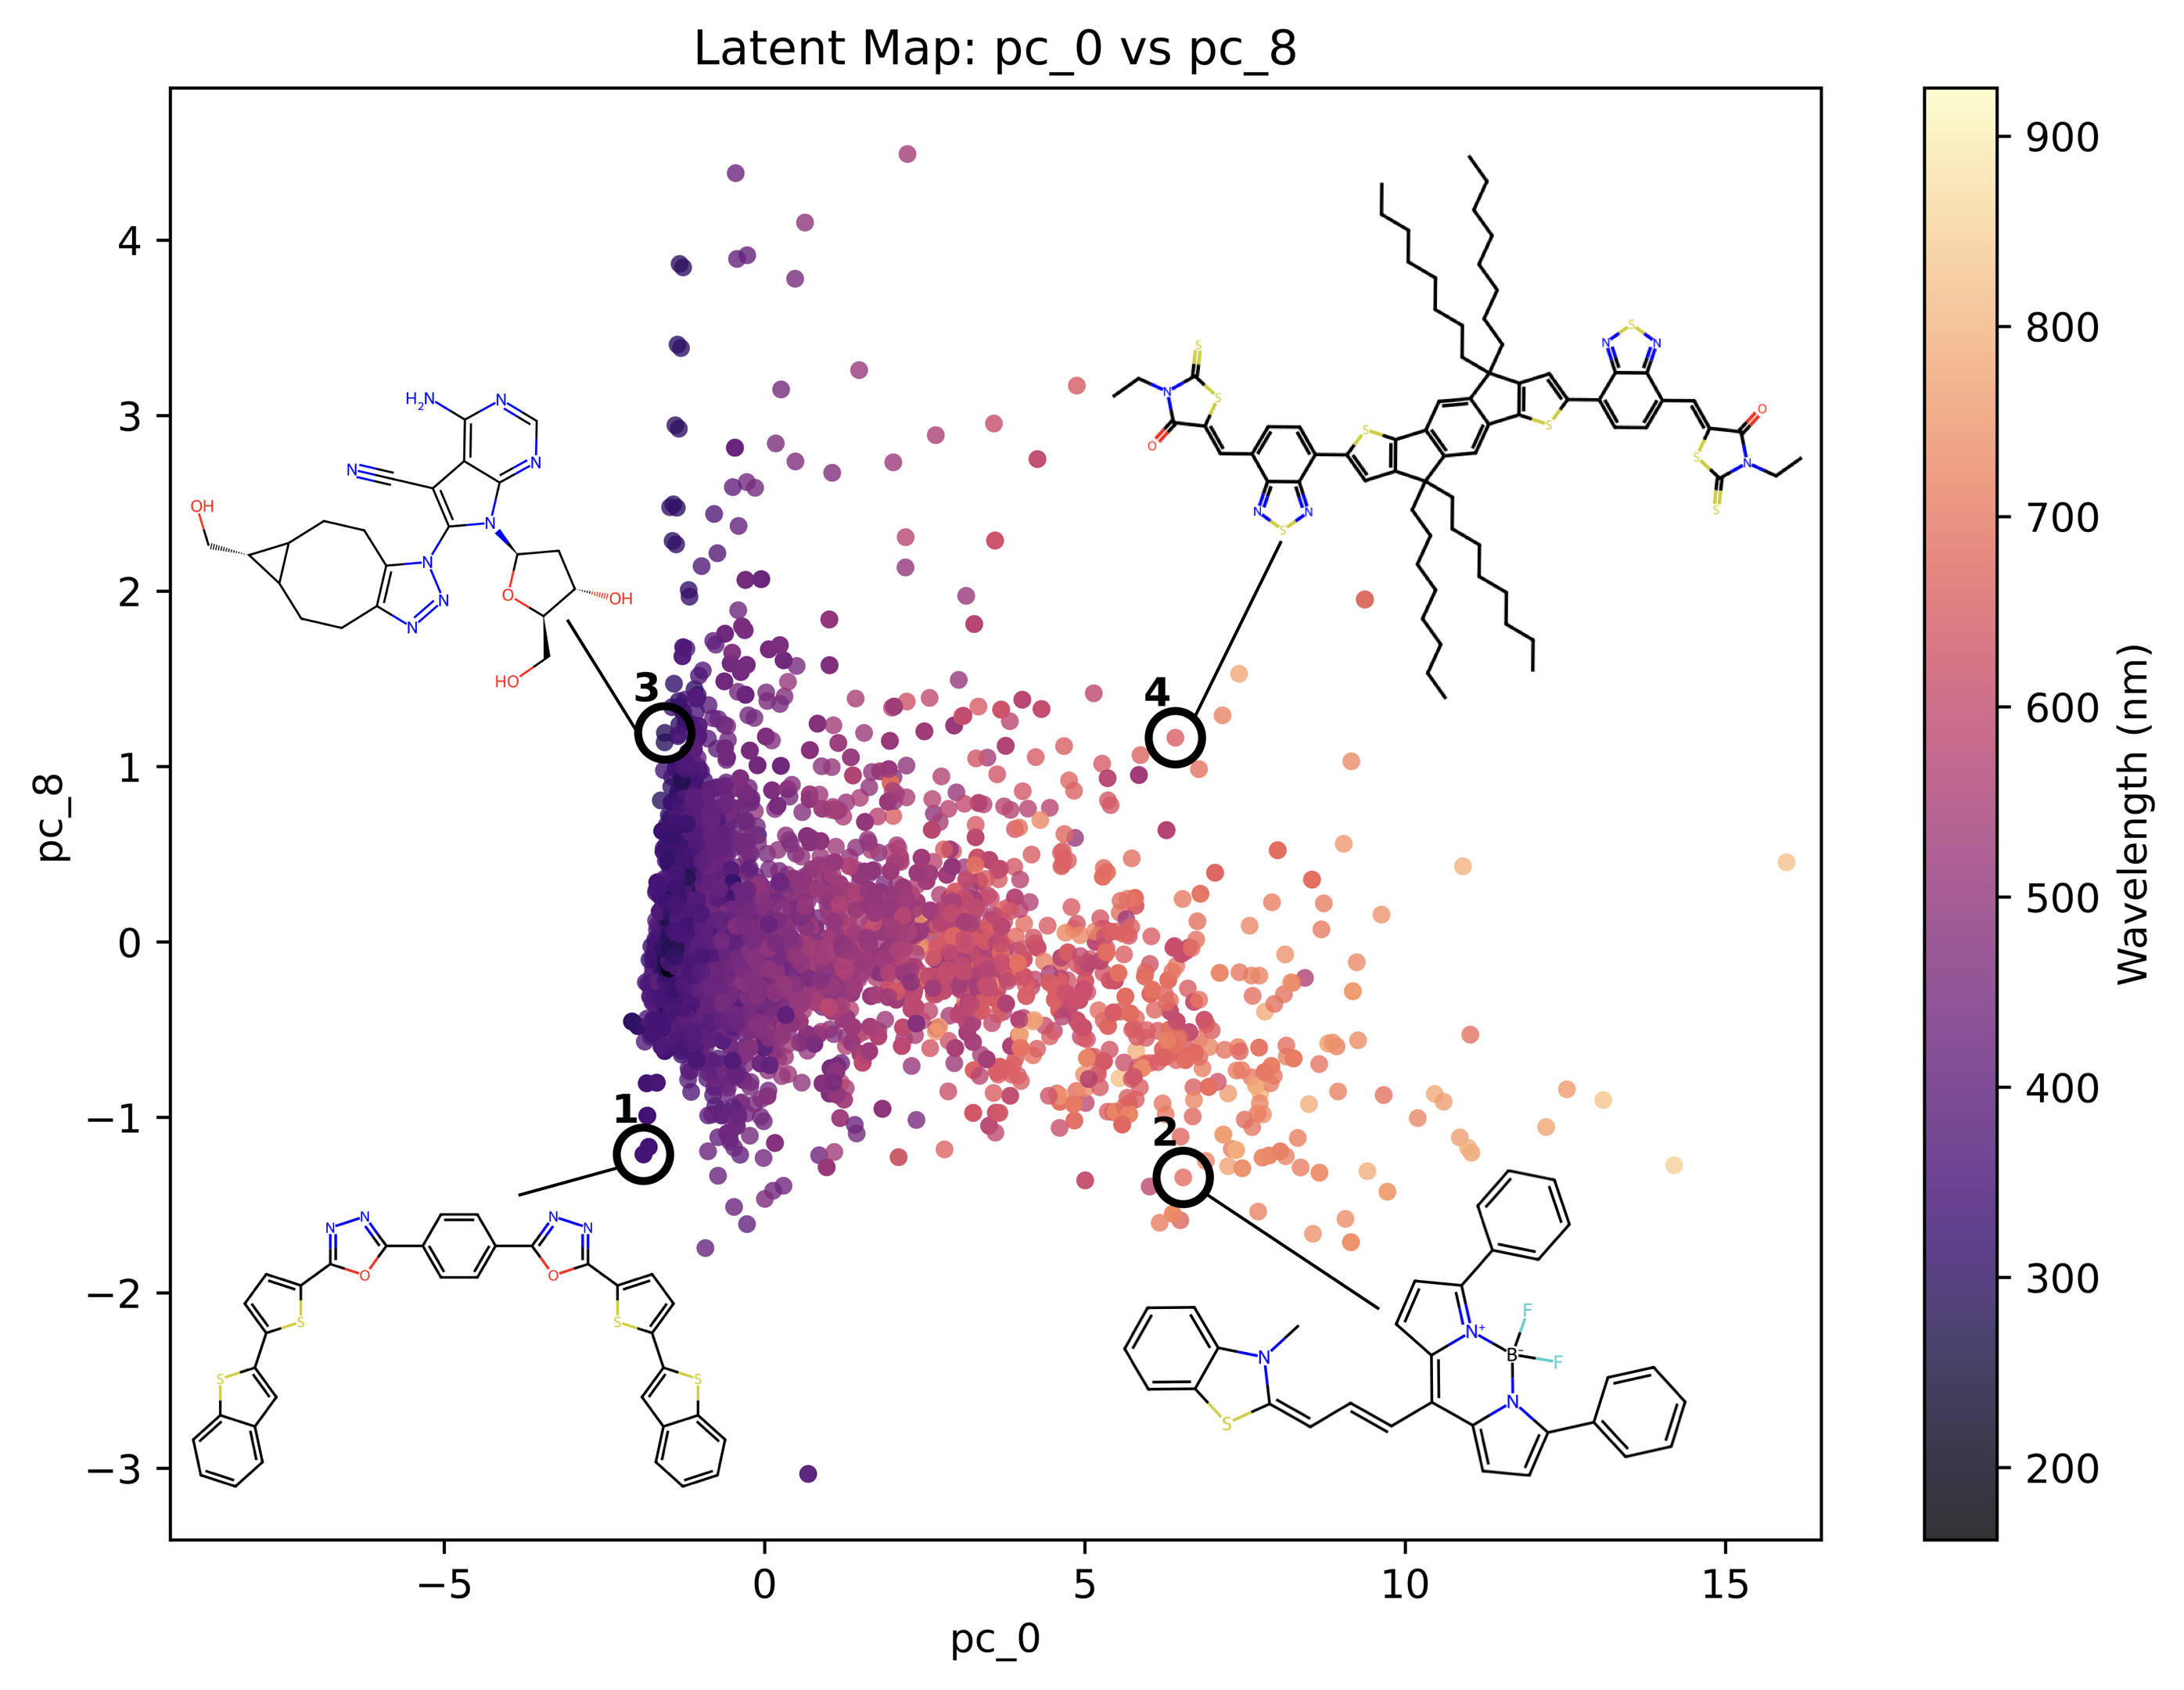
\includegraphics[width=0.9\textwidth]{figures/pc8-pc0.png}
  \caption{\textbf{Latent manifold visualization of $PC_8$ (Polarity and Solvation axis) versus $PC_0$ (Effective Conjugation axis).} The embedding successfully separates the electronic drivers of absorption (horizontal shift) from the structural ballast governing polarity and solvation (vertical shift). Representative molecules highlight the transition from rigid, non-polar systems (bottom) to highly substituted, polar, or branched architectures (top).}
  \label{fig:pc8-vs-pc0}
\end{figure*}

\FloatBarrier

\subsection{SHAP Attribution Analysis}

Finally, to connect geometric structure with predictive behaviour, we analyze feature attributions using SHAP values. The SHAP analysis aligns with the principal component interpretation. $PC_0$ dominates the predictions and shows a smooth, monotonic relationship with $\lambda_{\max}$, consistent with its role as the main driver of spectral shift. Higher-order components contribute smaller, more localized effects, suggesting that they capture secondary factors such as polarity and substituent-driven perturbations. Overall, the model appears to rely on a small number of structured latent features rather than diffuse correlations.
\begin{figure*}[ht]
  \centering
  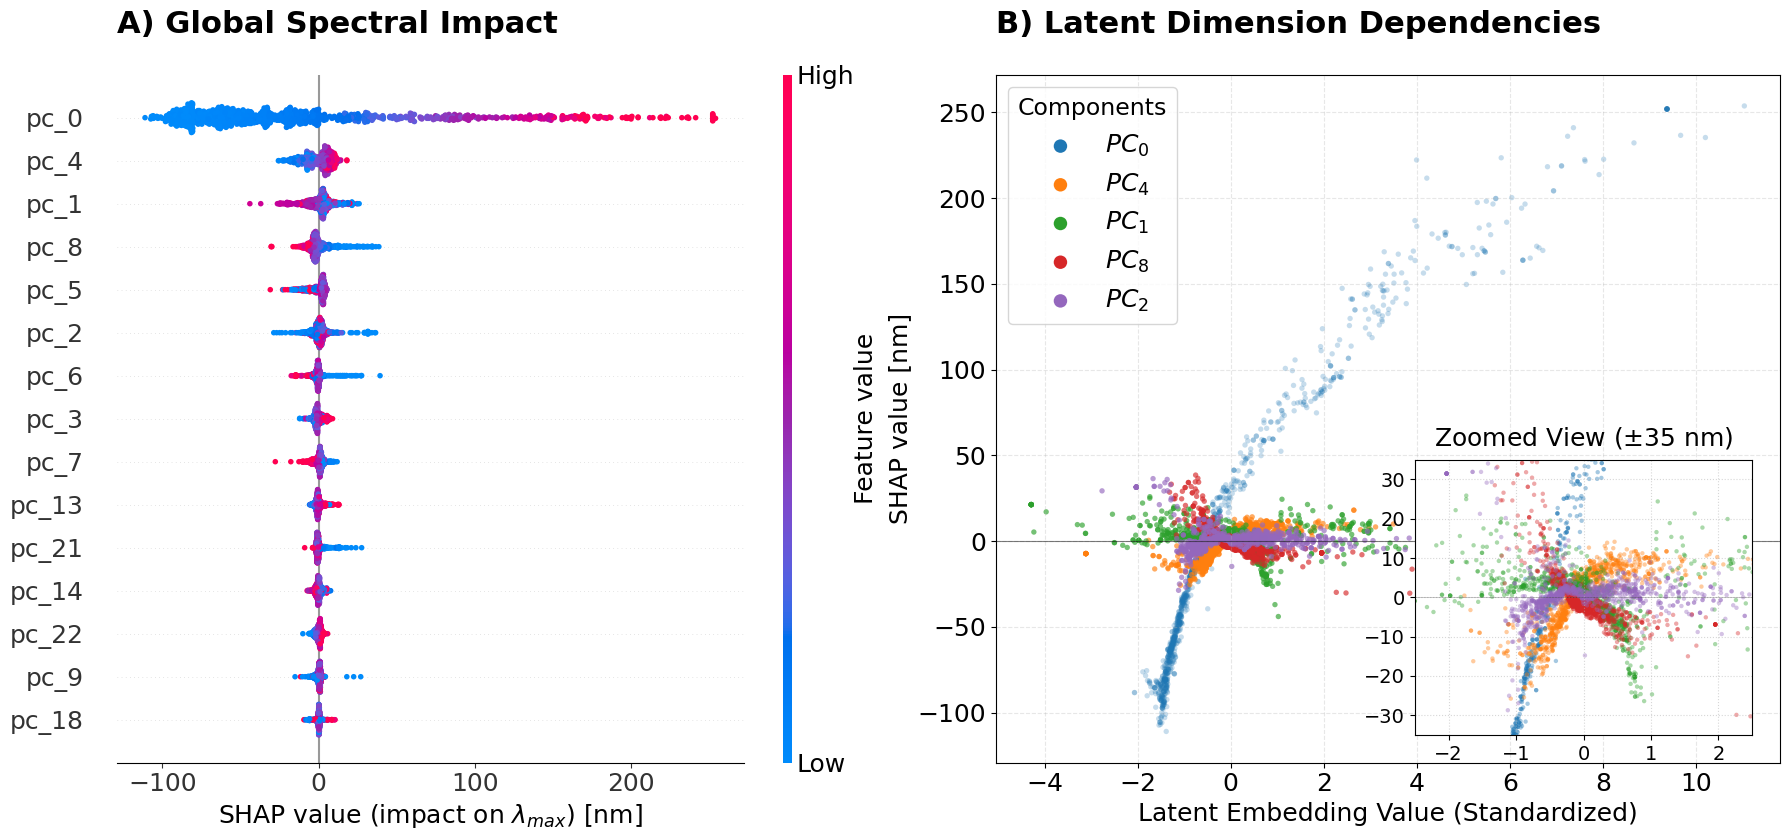
\includegraphics[width=0.9\textwidth]{figures/shap-scores.png}
  \caption{\textbf{Interpretation of the learned latent representation via SHAP values.} (A) SHAP summary plot showing the relative contribution of principal components to predicted $\lambda_{\max}$, with $PC_0$ dominating the global spectral shift. (B) SHAP dependence plots illustrating how latent dimensions are used by the model: $PC_0$ exhibits a smooth, monotonic relationship with absorption wavelength, while higher-order components contribute smaller, localized, and non-linear adjustments (inset, $\pm$35 nm).}
  \label{fig:shap-scores}
\end{figure*}